
% !TeX spellcheck = en_GB
\documentclass[]{article}
\usepackage{graphicx}
\usepackage{csquotes}
\usepackage[english]{babel}
\usepackage[hyphens]{url}
\usepackage{bookmark,hyperref}

\hypersetup{
	pdfauthor={},
	pdftitle={Blockchain-based provably fair data commerce with representative sample checking},
	pdfsubject={},
	colorlinks=true,
	linkcolor=black,
	citecolor=black,
	urlcolor=black
}
\usepackage[backend=biber,hyperref=true,backref=false,style=numeric]{biblatex}
\bibliography{../bib/data}

% \addbibresource{main.bib}
%\bibliographyystyle{}
%opening
\title{Blockchain-based provably fair data commerce with representative sample checking}
\author{}

\begin{document}
	
	\maketitle
	
	\begin{abstract}
		When buying a database, its difficult to get a fair idea of its value without actually seeing the data or having preexisting trust in the data provider. Our protocol solves this problem by using probabilistic verification: a chunk of the database is shown to the potential buyer in order for him to make an assessment about the data value. By leveraging blockchain technology as a trusted thrid party, it guarantees the revealed data is random sampled so the buyer is not cheated and that the seller receives the money once the buyer has received the database.
	\end{abstract}
	
	\section{Introduction}
	The use of data within a business has become an increasingly important aspect to the business success. Research has shown that proper use of big data techniques helps identify new insights, optimize operating processes and take better and faster decisions. In this context, ecosystems have grown to fulfil the data needs of diverse actors in the market: data suppliers, data custodians, data aggregators... 

Therefore, players in the market not only collect the data they are generating and analyse it, but increasingly rely on third party data to enhance its business value. The remaining challenges of the sector are, notably, regulatory complexity, privacy, the difficulty of making proper data agreements and the difficulty of valuing data and convincing customers of its value without giving it away \cite{thomas16}.
	
The creation of marketplaces addresses many of this problems. It helps to join interests between providers and consumers in a platform where both parties can meet each other and trade information. It solves the integration problem of connecting users and providers; however, some other drawbacks still remain. This work will focus on the problem of convincing consumers of data value, which can be seen as a form of lack of trust in data providers: a problem that still cannot be solved without previous confidence establishment. It manifests mainly as an entry barrier to providers in the market [27], hurting competence and thus reducing utility for consumers. A protocol will be presented to address this problem in a data trade, while preserving the necessary security, privacy and fairness characteristics that a marketplace should have.

	%TODO AÑADIR REFERENCIAS:
	%[26] 	L. D. W. Thomas and A. Leiponen, “Big data commercialization,” IEEE Engineering Management Review, vol. 44, no. 2, pp. 74-90, 2016. 
	%[27] 	Z. Feng and M. Iansiti, “Entry into platform-based markets,” Strategic Management Journal, vol. 33, no. 1, pp. 88-106, 2012. 

	\section{State of the art}
	A standard solution for trust establishment/maintenance is to use identifying information, since requiring e-mails, credits cards and other data constitutes an entry barrier to fraudsters. In pure data markets, being essentially business to business, it is even more feasible to demand identification warranties. In some cases, it can be also used as a negative incentive by, for example, recurring to law enforcement if tangible fraud is committed. These are however tedious and expensive processes and may not be feasible when the problem is that the quality of the data is not fulfilling expectations.
	
	From a consumer/client perspective, credit card payments often work as a hidden escrow service in e-commerce, as there are many options to get reimbursed if fraud occurs. Reputation systems are also a common way to penalize perceived malicious actors and reward legitimate ones, for example with more visibility. 

	Normally a combination of all these techniques is used in successful e-commerce websites [26]. However, these methods are incompatible with anonymity. On top of it, they pose entry barriers for new actors.

	\section{Data Exchange with Random Verification}
	Achieving the exchange of virtual products with many parties while minimizing risks is the main goal of virtual commerce. In order to exchange value safely it is essential that i) consumer is getting the product that it is paying for and ii) provider is paid. This is achieved, many times, without any strict protocols, just by existing trust. Counterparties know each other and are confident, by previous experience or by future interest, that no intent to scam will be made by other parties. When stronger assurance than that provided by direct mutual trust is needed, a trusted third party (TTP), whom all the parties trust, guarantees the process is carried out to all parties. It solves the crucial aspect of minimizing risk but comes with an extra cost for all parties and the need for a viable TTP.
	
	In general, Distributed Ledger Technologies (DLTs) can be seen as a paradigm shift when it comes to the need of trusted third parties for something as critical as payment processing. The use of public-key cryptography provides strong assurance and easy verifiability when attributing actions (payments) to specific participants (cryptocurrency owners). Using DLTs, all participants in the network can maintain a synchronized version of a database (who owns what) without the need for a central authority (TTP) that guarantees integrity, fairness or availability. 
	
	The protocol hereby presented for data exchange shares the goals previously stated for virtual commerce. It also provides a solution to the lack of trust in data providers, and the data they provide, conceptually different from those explained before: offering a sample of the data to the consumer. Therefore, its goals are:
	
	\begin{itemize}
		\item That the consumer gets a fair sample of the data being traded before committing itself. The protocol must ensure that the whole data is statistically consistent with this sample and so that the sample is not influenced by the provider. Thus the consumer can assess its value realistically.
		\item That the provider is paid, if and only if, the consumer has access to the data. Thus the transaction is correct: the consumer cannot get the data without paying and the provider cannot get paid without giving away the data.
		\item That the solution is cost efficient. Thus the cost of running the protocol is much smaller than the value of the data it can trade. Due to high fees on public ledgers, the cost of the designed solution must remain mostly fixed and amount of data saved on the network mostly independent of the quantity of real data traded.
	\end{itemize}

	\subsection{Design of the protocol}
	The design presented here is for selling a set of non-real-time data, although the protocol can also work with a flow of real-time data by paying for batches of real-time data, obviously with some delay that must suit the service policies. The design rationale of our solution is depicted next and more details are provided in subsequent sections.

	The protocol begins by generating a sequence of encryption keys to create a set of cryptograms that result from sequentially encrypting the fragments of clear data with the generated keys.

	The provider delivers the complete set of cryptograms to the consumer. Obviously, it would be totally impractical to exchange that amount of data using the ledger as a storage. Instead, the exchange of cryptograms between the provider and consumer is done off-blockchain. This approach is completely aligned to the current BIGIoT philosophy of direct connections between providers and consumers which is clearly stated in Deliverable D2.4 and also followed in the approach presented in Section 1.

	Next, the provider deploys a SC in a ledger that stores the root of two merkle hash trees. One root is the root of the tree formed hashing the cryptograms and the other root is the one resulting from hashing the keys. A merkle tree [28] is a structure that allows for efficient and secure verification of content in a large body of data. This structure helps verify the consistency and content of the data.

	Commitments using root hashes are very efficient, in this case, since two hashes are stored in the ledger. These roots will allow to prove whether an element is or is not a cryptogram or a key and its position in the merkle tree. Using this, we will be able to assure to the consumer that the provider cannot alter the committed data set.

	Then, some encryption keys are revealed by the provider in order to disclose a fair data sample that could convince the consumer about the value of the data set. At this moment, it is very important for the producer to make sure that, with the set of disclosed keys, it is not possible for the consumer to derive any previous or posterior keys of the sequence of keys used to encrypt the data; although the consumer must be able to easily derive all the keys when it agrees to buy the data set. A simple way to get this is to create the keys as hashes of a (initially private) seed and the index of the key in the sequence. This construction has the properties that we want: without the seed, the consumer cannot derive any other keys but once the seed is known, it is easy to regenerate the sequence of keys. Notice also that, since the seed will be public at the end of the process, all the off-blockchain traffic including cryptograms must have been exchanged using a secure channel.

	Another important issue that our protocol has to solve is how to select and exchange the keys to disclose the fair data sample. The important aspect here is that the provider cannot control this process because, if this happens, the provider could decide to use a biased (not fair) data sample. Then, we have two options, either let the SC decide the indexes to be disclosed and or let the consumer decide them. We use the second option because then, the selection and exchange can be done totally off-blockchain. Doing this on-blockchain requires the availability of a random selection algorithm within the SC, which is not a trivial issue for distributed ledgers.

	Since getting the sample has no cost for the consumer (it is off-blockchain), a potential attack could be a consumer trying to get a large amount of free data by repeating the process of getting small samples. In such a case, the provider can decide how many times it allows getting a sample set without making a final deal and it can use the marketplace to blacklist abusive consumers.

	Finally, if the fair sample convinces the consumer, it will send a transaction to the corresponding SC with the payment to buy the data. Then, the provider discloses the seed that allows the consumer to derive all the keys, decrypt the previously received cryptograms and access the data. If everything is OK, the protocol ends after some time by sending the payment to the producer or by letting the producer withdraw the payment.

	The final aspect that our protocol has to solve is when the provider either uses incorrect keys (keys that do not correspond to the sequence generated by the seed) or sends incorrect cryptograms. In both cases the consumer will be unable to decrypt a set of cryptograms to obtain the data. For such a reason, our protocol adds an optional final step that could be used to resolve conflicts by allowing the consumer to challenge the provider to proof that it sent a valid key for a given valid cryptogram. Conflict resolution an exceptional situation that is, in general, discouraged because it has costs for either the consumer or the provider.

	When the subscription is created, the provider locks an amount of crypto currency that could be used to execute the conflict resolution. If the consumer is not able to decrypt a cryptogram (either because of an incorrect key or an incorrect cryptogram), the consumer executes the conflict resolution on the SC. If the provider cheated, the SC will refund the consumer and the cost of the execution will be charged to the provider by unlocking the money locked for conflict resolution. If the provider didn’t cheat, the consumer will have to pay the execution of the conflict resolution in the SC, so that there are not incentives for a consumer to cheat.

	Although explained and detailed below, for reference purposes Figure 12 pictures the protocol operation and the interactions between the different stakeholders and the SC. Moreover, Table 3 summarizes the notation in use.

	We assume a marketplace model similar to Section 1, in which offerings are stored via SCs on the DLT. Figure 12 does not repeat the full marketplace concept from Section 1 but instead focuses on the interaction with the SC during the search and presubscription phase. Red text in the figure denotes calls to SC functions, the ovate shapes represent the different states of the SC.

	% TODO ESQUEMA GENERAL D'ESTATS I FASES, SEPARANT EL QUE VA PER SC y OFF-BC
	The notation in the protocol:
	%TODO Crear tabla con este contenido
	\begin{itemize}
		\item $D = d_1 ... d_n$: data samples
		\item $s$: cryptographically secure random number for key creation (salt)
		\item $K = k_1 ... k_n$: encryption keys for data samples, such that $k_n = Hash(n + s)$
		\item H(K): root of the Merkle hash tree containing all generated keys
		\item Cn: encrypted data samples, such that EKn(Dn) = Cn
		\item H(C): root of the Merkle hash tree containing all encrypted samples
		\item N: number of data samples
		\item V: number of data samples to be revealed
		\item Rn: indexes of the samples to be revealed
		\item P: price
		\item paymentA: price that A must block in order to prevent multiple SC creation
		\item paymentB: price that b must pay in order to not get samples for free
		\item MP: Merkle proof. Merkle hash tree leaves needed for an auditor to verify an item is inside a Merkle hash tree knowing only its root.
	\end{itemize}
	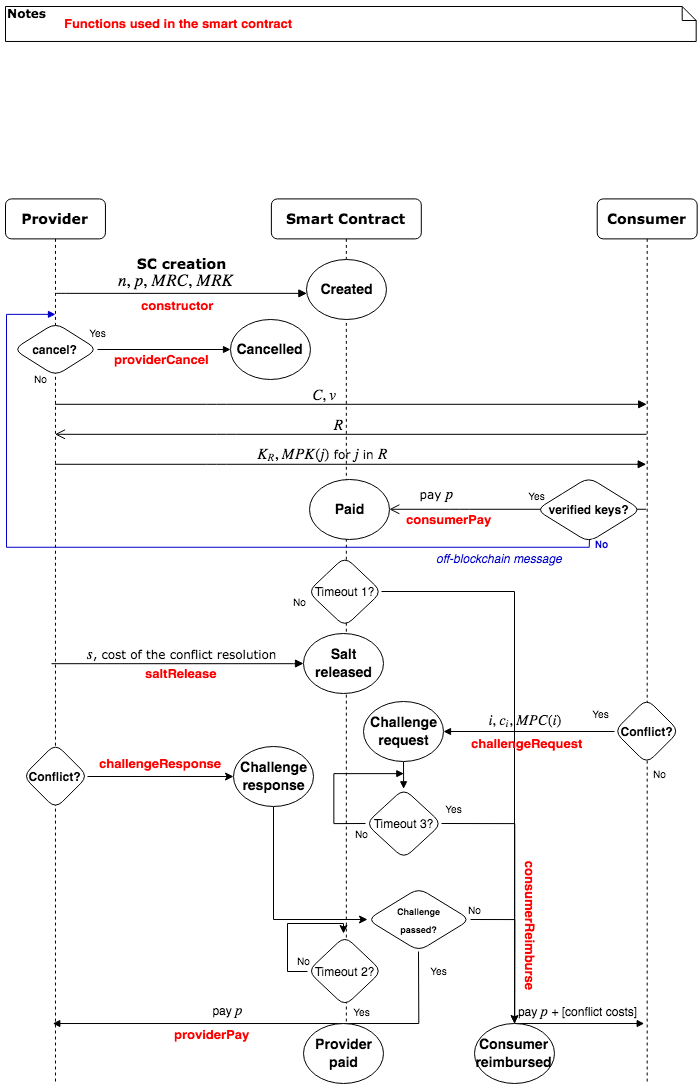
\includegraphics[width=\textwidth,height=\textheight,keepaspectratio]{../figures/Diagram_InteractionSC}

	
	\subsubsection{Step 1. Data preparation and SC creation (provider)}
	The provider must prepare the data, splitting it in different samples. There will be cases where data splits “naturally” (e.g. records of a database, where each record is a sample) and others where samples must be generated from a compact source of data (e.g. video). Data must be sorted, using the most valuable variable, in case there are multiple ones. This will avoid a potential attack explained in Section 3.4.

	A random seed number, s, must be generated in order to create the keys that will encrypt each sample of the whole data separately. Once data is split into different samples and a seed is created, the provider must create two merkle hash trees:
	
	\begin{itemize}
		\item Merkle tree of encrypted data: each leaf will be an encrypted data sample ci. An example is shown in Figure X.
		\item Merkle tree of keys: each leaf will be the key that deciphers the same element in the Encrypted data merkle tree. An example is presented in Figure 14.
		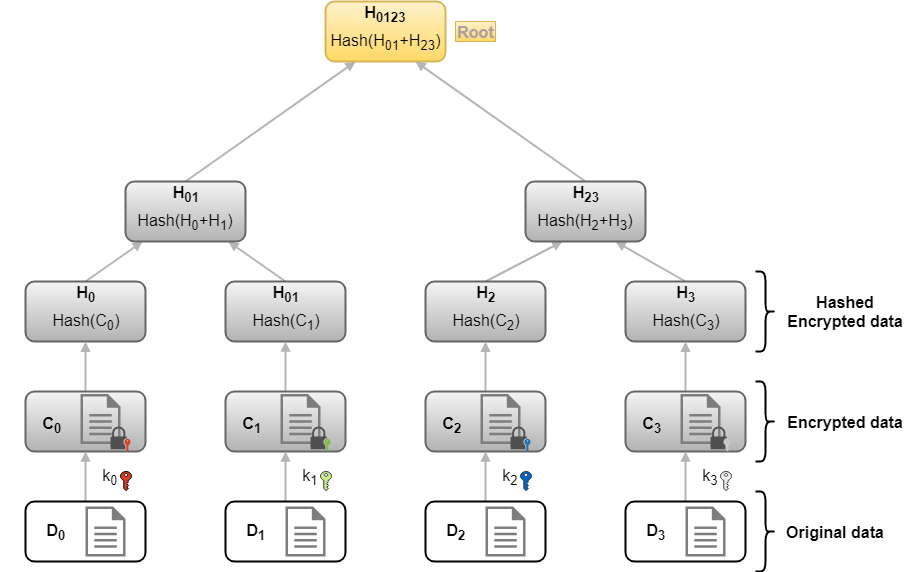
\includegraphics[width=\textwidth,height=\textheight,keepaspectratio]{../figures/MerkleTree_EncryptedData}
		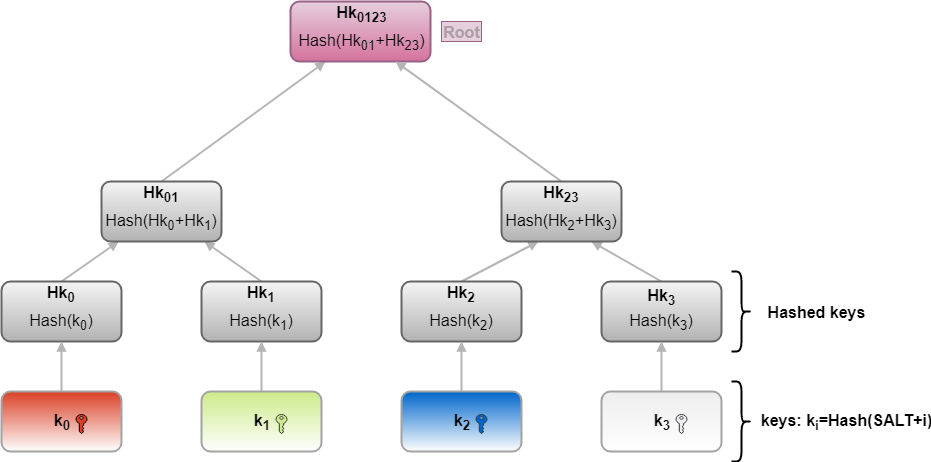
\includegraphics[width=\textwidth,height=\textheight,keepaspectratio]{../figures/MerkleTree_Keys}
	\end{itemize}
	
	Now the provider must deploy a public SC showing the specifications of the data offered, including a description of the data offered, the price of the whole data and the total number of samples it consists of.
	
	\begin{itemize}
		\item (Provider$\rightarrow$SC) n: the total number of samples.
		\item (Provider$\rightarrow$SC) p: price of the data willing to sell.
		\item (Provider$\rightarrow$SC) MRC: the root of the encrypted data merkle tree of the encrypted data. In addition to its use in the protocol, it will act as a check that bulk data was received correctly.
		\item (Provider$\rightarrow$SC) MRK: the root of the keys merkle tree of the keys that encrypts each sample.
	\end{itemize}
	
	\subsubsection {Step 2. Data shipping (provider)}
	Once a consumer has made contact, the provider sends off-blockchain:
	\begin{itemize}
		\item (Provider$\rightarrow$Consumer) C={ci}: all data samples encrypted.
		\item (Provider$\rightarrow$Consumer) v: number of data samples to be revealed.	
		%\item (Provider$\rightarrow$Consumer) H(C): the root of the encrypted data Merkle tree. In addition to its use in the protocol, it will act as a check that bulk data was received correctly.
		%\item (Provider$\rightarrow$Consumer) H(K): the root of the keys Merkle tree that encrypts each sample.
	\end{itemize}
	These items do not provide any relevant information about the data to the consumer, other than already known aspects such as size. The off-blockchain channel used has to be encrypted to avoid a potential attack explained in Section X. 
	
	\subsubsection{Step 3. Selection of the samples to be revealed (consumer)}
	Once the buyer has checked he received the information correctly, he sends to the seller and the smart contract:
	\begin{itemize}
		\item (Consumer$\rightarrow$Provider) R: indexes of the samples the consumer wants to check. Notice that they will be random samples because the consumer does not have any information about the data.
	\end{itemize}
	
	\subsubsection{Phase 4. Sample keys revelation (provider)}
	The provider sends to the consumer: 
	\begin{itemize}
		\item (Provider$\rightarrow$Consumer) $K_R$={$k_j$}  ∀  j∈R: the keys that decipher the samples that B has chosen.
		\item (Provider$\rightarrow$Consumer) {$MPK(j)$}  ∀  j∈R: the merkle proofs  that ensure these keys are part of the original key tree, and so have not been altered.
		%Merkle proofs and KRv provides the root H(K).  
	\end{itemize}
	
	\subsubsection{Phase 5. Payment (consumer)}
	Now, the consumer has all the information needed to make a decision on whether to buy the data or not. Protocol-wise, all he needs is to make sure the keys revealed correspond to the original key tree by using the merkle proofs. Not doing so would make him vulnerable as the decrypted samples may not correspond to the data set. As to whether the information in the whole data is worth the price, the question goes beyond the scope of this paper.
	\begin{itemize}
		\item (Consumer$\rightarrow$SC) payment. o	SC triggers Timeout 1: if the provider does nothing, the consumer is reimbursed and the protocol ends; otherwise the providers gets paid once the timeout triggers.
	\end{itemize}
	
	\subsubsection{Step 6. Salt release (provider)}
	Once the consumer has made the payment, and thus has shown interest to buy the data:
	\begin{itemize}
	\item (Provider$\rightarrow$SC) cost of executing the conflict resolution in the DLT native crypto currency. In order to guarantee a fair potential conflict resolution in the future, the provider locks some money in the SC that could be used to execute the conflict resolution if the provider cheats.
	\item (Provider$\rightarrow$SC) s: the random seed from which the keys for each index have been created.
	\end{itemize}
	Now the consumer has access to the key generator and can decrypt the data, it will just check that the sample keys, provided in step 4 for the indexes chosen in step 3, have been truly generated using this random seed, as explained in step 1.

	If the result is positive, the provider is guaranteed not to have cheated. In this case, the consumer should not do any further action and the payment to the provider will happen once the timeout triggers. 

	If it is not possible to obtain all the sample keys with the salt, there exists no guarantee that the samples come from the full data. In this case, the provider should challenge the consumer to prove its honesty and two optional steps are required for conflict resolution. To put time limits to those actions, the:
	\begin{itemize}
		\item SC triggers Timeout 2: if the consumer does nothing, the provider gets the payment and the protocol ends.
	\end{itemize}
	
	\subsubsection{[optional Phase 7] Conflict resolution: specific key challenge (consumer)}
	Once the consumer finds a key that could not be used to decrypt an encrypted data sample (either because of an incorrect key or incorrect cryptogram), it provides its index to the SC and the affected encrypted data sample. This step obviously has a cost that must be paid initially by the consumer to the SC.

	\begin{itemize}
		\item (Consumer$\rightarrow$SC) i: failing key index.
		\item (Consumer$\rightarrow$SC) Ki: failing key.
		\item (Consumer$\rightarrow$SC) MPK(i): the merkle proof for the affected key (can be checked against the already published MRK).
	\end{itemize}

	The SC will check: 
	\begin{itemize}
		\item $i$ is coherent with $MPK(i)$.
		\item $k_I=H(S+i)$.
		\item $MPK(i)$ and $k_I$ are coherent with MRK.
	\end{itemize}

	And resolve:
	\begin{itemize}
		\item If the first two checks work and the third does not, all the payments done by the consumer are reimbursed.
		\item In any other case, the seller gets the payment.
	\end{itemize}
		
	
	In order to track the index of each key, the merkle proofs must be used taking into account the concatenation side. In figure X, each index is converted to binary and each digit indicates if the merkle proof must be concatenated on the right side (0) or in the left side (1).
	
	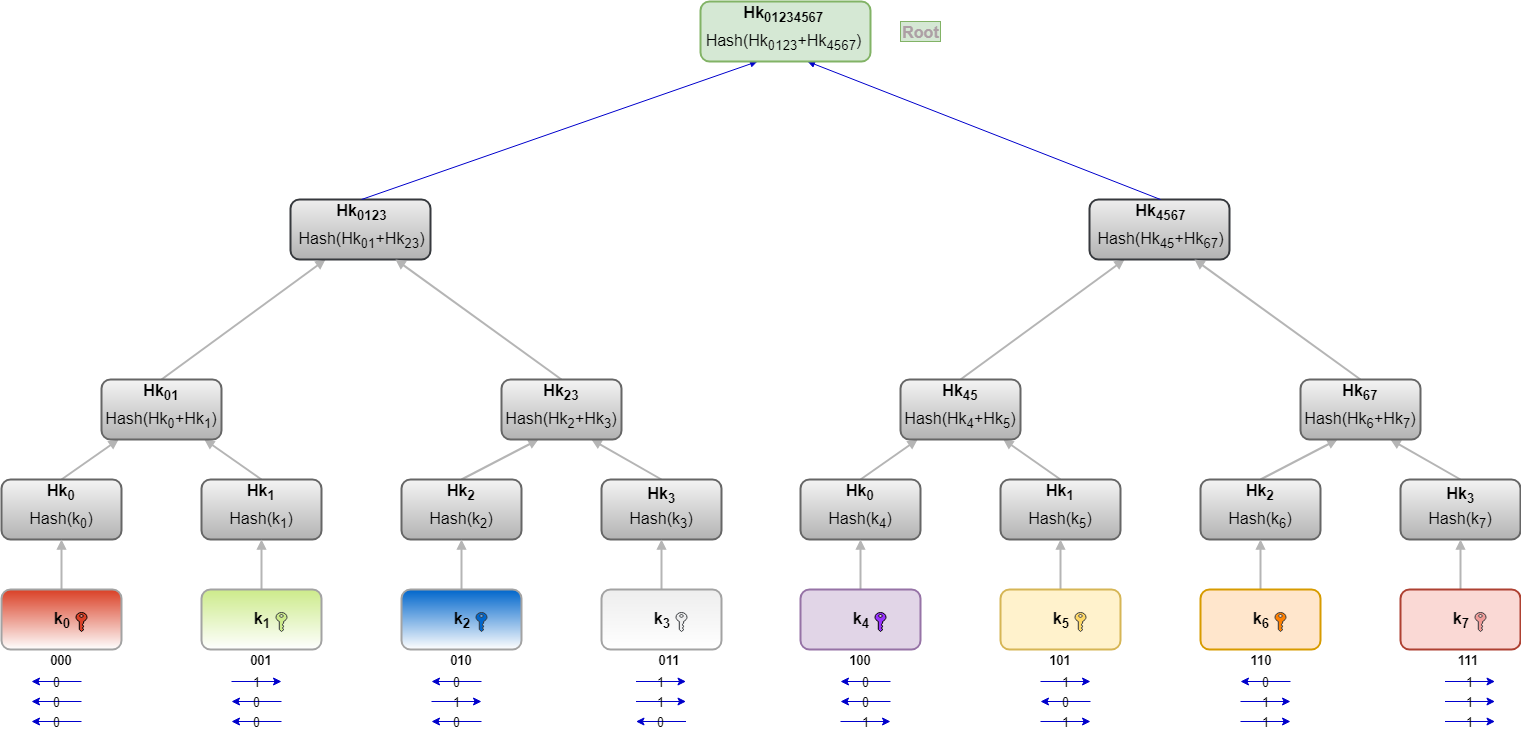
\includegraphics[width=\textwidth,height=\textheight,keepaspectratio]{../figures/KeysMerkleTree_index}

	\subsection{Protocol's improvements}
	Adding format to the data could disjoin the data quality checking from the keys authenticity. The consumer could realize whether the data was originally useless or the key used to decrypt the sample was not working.
	Applying format could provide a consumer the ability to report to the smart contract an invalid key generated by the salt. For it, the consumer must send the smart contract:
	\begin{enumerate}
		 \item index
		 \item the $k_i$ to report and the merkle proofs that demonstrate the inclusion of $k_i$ in the keys merkle tree
		 \item the $c_i$ and the merkle proofs that demonstrate the inclusion of $c_i$ in the cryptograms merkle tree
	\end{enumerate}
	
	The smart contract will check that both $k_i$ and $c_i$ are committed to each merkle tree and prove that the deciphered $c_i$, $d_i$, has the correct format. The merkle proofs will be used taking into account their side to concatenate as previously explained in last section.
	
	
	\section{Protocol's implementation}
	
	\subsection{Ethereum's network and development settings}
	Ethereum network is a decentralized platform that enables the execution of smart contracts (SC) [REF1]. Smart contracts are autonomous programmed applications that are built on top of a custom blockchain [REF2], run without any censorship or third party interference and allows to avoid a counterparty risk. Therefore, it provides a perfect ecosystem to implement a two-way protocol requiring trusted identification, neutral execution of previously agreed-upon checks and payment processing.
	Environment used to deploy and test the solution: Ganache, Metamask, nodejs...
	%TODO Mirar las diapos del postgrau i comentar un poco.
	
	\subsection{Smart Contract solution}
	Posar aqui la version final del SC. Optional: fer algun diagrama per veure com interactuen el byuer i el seller amb l'SC veient els estats en els que pot estar el SC: Created, SampleRequested, SampleProvided, SampleGenerated, Paid, InactiveNotSample, InactiveOK, InactiveKO, InactiveAbortedS, InactiveAbortedB

	\subsection{Choosing revealing sample size}
	The optimal size of the revealed sample depends on the nature of the data. Mainly, it should be big enough for the buyer to be fairly sure the data is worth the price, given the random nature of the sample selection. Here we provide a working example where the value of the data is binary. This could easily be the case in a simple e-mail database, where the only relevant aspect of a record is if the mail is responsive for advertising or not.
	Given the level of precision (D) at a desired level of confidence (z), the minimum sample size to estimate the proportion of responsive e-mails (being $\pi$ the true proportion) is:
	
	%For mean estimation:
	%\begin{equation}
	%n =  o^2 z^2/ D^2 
	%\end{equation}             
	%(o = true sigma)
	\begin{equation}
	V = \pi(1-\pi)z^2/D^2
	\end{equation}   
	
	Therefore, having a database with 30\% of responsive e-mails, to give the buyer a 95\% confidence on estimating this proportion between 25\% and 35\%, the seller should choose a revealed sample size of: 
	\begin{equation}
	V = 0.3(1-0.3)(1.96)^2/(0.05)^2 = 323
	\end{equation}  
	%A correction exists not(V>>N):
	%\begin{equation}
	%n_c  = \frac{nN}{N+n+1}
	%\end{equation}     
	%(N = population size)
	
	As explained in (Potential attacks, 3-4), without complicating the protocol further, the revealed sample size should also be small enough that the buyer has no incentive to ask for the sample just to obtain it's data without buying. It should also be big enough that the seller has no incentive to repeat the protocol until a buyer chooses a good sample set.
	
	%pag 228 9.4a 9.4b 9.6
	
	%https://books.google.es/books?id=xLq8BAAAQBAJ&pg=PA229&lpg=PA229&dq=database+marketing+optimal+sample+size&source=bl&ots=6fuwwKVeBl&sig=CQ-WNf4mSPTIZKZh2ImglTYyckI&hl=es&sa=X&ved=0ahUKEwjIoc2hz7vaAhWKWBQKHRG8B_sQ6AEILTAA#v=onepage&q=database%20marketing%20optimal%20sample%20size&f=false
	
	\section{Potential attacks}
	\subsection{Eavesdropping - in Phase 2 - by an external party}
	A potential attacker eavesdropping the channel between consumer and provider could get a copy of the cryptogram. Thus, if the protocol finishes correctly, the s will be revealed and he could get access to the data for free. To prevent it, the channel must be encrypted as stated earlier. For the same reason, if during a protocol run the consumer receives the cryptogram and then cancels, this cryptogram and the associated SC cannot be reused another time.
	
	\subsection{Data Replication - in Phase 1 - by the seller} When the value of the data in a dataset is not linear, as is the case in an email database, where duplicated samples are worth nothing, an attack is possible: the provider could make many replicas of the data and merge them. If the amount of different samples before replication is big enough, the samples revealed to the consumer will all be provably different. Thus, the consumer will not get a fair idea of the database content. To avoid this problem, the consumer should get confident that the data are sorted using the most meaningful variables; e.g. by asking for some sets of consecutive samples, which may help to estimate the data replication ratio.
	
	\subsection{Offer Replication - in Phase 1-3 - by the seller} 
	As the consumer performs the data evaluation with a reduced amount of random samples, there exists some variability on its value perception. Consequently, a malicious provider could try repeating the selling process multiple times until the samples chosen are good enough for the consumer to accept the trade. The variability of the value perception in the sample sets depends exclusively on the amount of samples. Therefore, the consumer must ensure there are enough samples provided so that it is not profitable for the provider to repeat the process multiple times, given the fixed costs of the SC creation. Another possible solution would be for the provider to block/burn some crypto value (e.g. Ethers) as a guarantee that the attack is not profitable for him, regardless of the sample amount.
	
	\subsection{Request Replication - in Phase 1-5 - by the buyer}
	In a similar way as in the previous attack, a consumer could engage in the protocol multiple times without any intention of buying the whole data, and accumulate free samples during the process. For this to be non-viable, the provider should ensure the value of a revealed sample set is small enough compared to the fixed costs of the consumer. Like in the previous case, burning/blocking some Ether could be an alternative solution.
	% tunning de la muestra
	
	
	\section{Properties achieved}
	\subsection {Simultaneous probabilistic verification}
	It is important to note that the probabilistic verification is not only accomplished for the quality of the data but also for the authenticity of the keys. 

	If the keys sent to the consumer in step 4 are not generated with the provided salt, the consumer will realize comparing the committed keys with the keys created using the salt. 

	On the other hand, notice that if there exist a committed key that (i) is not included as part of the verification set KR and (ii) that is not generated by the salt, then, when the consumer decrypts the corresponding cryptogram, it will get a useless sample. In this case, the consumer will not be able to distinguish between a situation in which the provider has encrypted the data with an invalid key (not generated by the salt) or has included a random (i.e.  non valuable) as sample. This situation can be fixed enforcing the samples to follow some type of format.

	\subsection {Efficiency}
	We consider our protocol fairly efficient because the amount of storage used in the blockchain is fixed and the amount of operations only proportional to the logarithm of the number of samples and only in the worst case.
	\begin{itemize}
		\item Amount of data transferred off-blockchain: O(N)
		\item Amount of operations in the buyer/seller: O(N)
		\item Amount of data stored in the blockchain: O(1)
		\item Amount of operations in the blockchain: O(1) without challenge, O(log2(N)) with challenge.
	\end{itemize}
	
	\subsection{Provable fairness}
	We consider the samples revealed have no inherent value, which should be close to true. The amount of data revealed this way is not proportional to the size of the whole data, it should just depend on its nature. Thus, if the whole data is big enough, the value of the revealed samples becomes negligible.
	
	\textbf{From the seller perspective}, the only way he could be cheated is if the buyer has access to the data and he still does not receive the payment. This cannot happen as the seller will only reveal the SALT once the payment is in the Smart Contract, and the Smart Contract will award him the money if it checks he has not deceived in any way with the keys. As previously stated, the Smart Contract is guaranteed to work as expected with very high provability. As the keys are hashes originating from a pseudo-random number, there is no viable way for the seller to obtain them, other than paying.

	\textbf{From the buyer perspective}, as he has checked the sample keys are contained in the key tree, once the SC checks the SALT and payment is done, all the key tree is provably guaranteed to have been generated the same way. The buyer will be able to decipher the whole data in the same way it has deciphered the samples, and those will necessarily be part of the whole. If the check fails, the buyer recovers the money. Again, the SC is provably guaranteed to work as expected. The buyer has chosen the revealed samples indexes while already having the cryptogram so, whatever information it decrypts before payment, has to provably be like the rest of the information.
	
	\subsection{Liveness}
	%The protocol incentivizes both parties to complete de process but it is not asynchronous, as one must wait each other response to keep on the protocol. Thus, the protocol can be stuck if one of the participants does not act. For avoiding this problem, both can always abort the process and finalize the protocol if it is the counterparty turn to act. Finalizing and killing the contract lets unblock the situation in spite of it avoids finalize the trade.
	After the SC is created, the provider can cancel it if no consumer comes. After the payment, the timeouts ensure the counterparty can finalize the execution favourably to her if the party expected to act does not do so in time. This way, being the economic incentives right, the protocol is guaranteed to enter some of the final states.
	\subsection{Timeliness}
	
	\section{Conclusions and future work}
	We have proposed a protocol for secure data exchange that makes use of SCs in a DLT. In our protocol the consumer can check a subset of the data before the actual payment and both the consumer and the provider are protected. The provider will be always paid if the data is released and the consumer will only pay if and only if the data has been properly received and the initial set of sample data addressed the expectations. By the time of writing this deliverable (July 2018), we are working on an Ethereum implementation of this protocol that is expected to be released on October 2018 and published as a journal article a few months later.

	A major enhancement to the protocol would be to redesign it in a way that the SC and the cryptogram could be reused. The first two steps of the protocol would only be run once and the sample selection would be the same for all potential consumers, bringing in many advantages. First, the costs would be reduced as only a SC would be used independently of the number of failed sale attempts. Second, the use of the same random sample would make essentially disappear the first three presented potential attacks. Third, offer replication and request replication would not be possible by design. Fourth, samples could be bigger as its value is only given away once to everybody. And sixth, eavesdropping would not be possible either as many people having copies of the cryptogram should not be dangerous. Proxy reencryption technology is something that we have to definitely explore in order to be successful implementing this major enhancement.

	If this redesign were not possible, some incentive system should be designed to avoid the attacks, as commented in their section. Fixed costs for buyer and seller actions could prevent offer/request replication. Also permissioning and other forms of censorship could be used, although they would defeat the main purpose of the protocol.

	A relatively easy improvement would be to use an extended version of the merkle trees that guarantees not only that some information is included in the tree, but also where it is placed in the tree. By doing this, the challenge part could be reduced from two steps to one. In place of the buyer challenging the seller to prove a correct key is in the tree, the seller would directly prove to the SC that a wrong key is in some specific position in the tree. It would be simpler, with less costs, and the buyer could do any complains wanted as he would be paying them entirely.
	
	Another future work is to design meaningful sizes of data samples for different types of data.


	
	\printbibliography
	
\end{document}

